% Provenance (never printed): see sources/outline_sources.md (Year 2: sedimentary basins;
% subsidence curves and backstripping; the stretching model). Stretching model after McKenzie
% (1978) as restated by Sheplev and Reverdatto (1998) and coded in pyBacktrack (EarthByte);
% backstripping after pyBacktrack's well module; North Sea after Sclater and Christie (1980);
% Michigan after Sloss (1982) and Crowe et al. (2009); the US Atlantic margin after Schlee et
% al. (1976), Poag (1979) and Lang et al. (2024); the Molasse after the chapter 13 rows.
% Curves and the invented well from figdata/bachelor-2/basins.py; exercise and problem values
% in the Book 4 scratch calculator calc/ch16.py.
\chapter{अवसादी द्रोणियों की तुलना}\label{ch:b2:basins-compared}

पूर्वी संयुक्त राज्य अमेरिका के तट के पास, महाद्वीपीय शेल्फ़ के नीचे, बाल्टीमोर
कैन्यन द्रोणी में कम से कम \qty{14}{km} अवसादी चट्टान है। ऐसे ढेर में खोदा गया एक बोरहोल
उसका इतिहास उलटे क्रम में पढ़ता है: वह जिस भी इकाई को पार करता है वह कभी समुद्र-तल थी, उस गहराई पर जिसे
जीवाश्म और अवसाद अंकित करते हैं, और तब से दबी और भिंची है। हर
तिथि-निर्धारित सतह की गहराई अवधसान के एक वक्र पर एक बिंदु है। फिर भी अधिकांश अवधसान स्वयं अवसाद के
भार से हुआ। द्रोणी को किसने बनाया, यह जानने के लिए उस भार को हटाना होगा,
परत-दर-परत। यह अध्याय दिखाता है कि कैसे, और परिणाम स्थलमंडल के बारे में क्या कहता है।
% ledger: poag79:bct, schlee76:atlantic

\begin{recall}
\textbf{पुस्तक 3 (स्नातक वर्ष 1) से}: अवसादी द्रोणी, अवधसान और विवर्तनिक अवधसान,
आवास-स्थान, यूस्टेसी; संपीड़न, डिकंपैक्शन और एथी का नियम, किसी परत की ठोस
मोटाई; अवसाद-भार, जो अवधसान को $(\rho_m - \rho_w)/(\rho_m - \rho_s)$ गुना प्रवर्धित करता है;
एयरी समस्थिति; स्थलमंडल और उसका जियोथर्म; महाद्वीपीय दरारें और निष्क्रिय किनारे।
\textbf{भौतिकी की पुस्तकों से}: ऊष्मा-समीकरण और उसके फ़ूरिए हल।
\textbf{\cref{ch:b2:alpine-orogen} से}: \omterm{def:b2:alpine-orogen:foreland}{अग्रभूमि द्रोणी}, \omterm{def:b2:alpine-orogen:foreland}{फ़्लिश} और \omterm{def:b2:alpine-orogen:foreland}{मोलास}।
\end{recall}

\begin{omfigure}
\centering
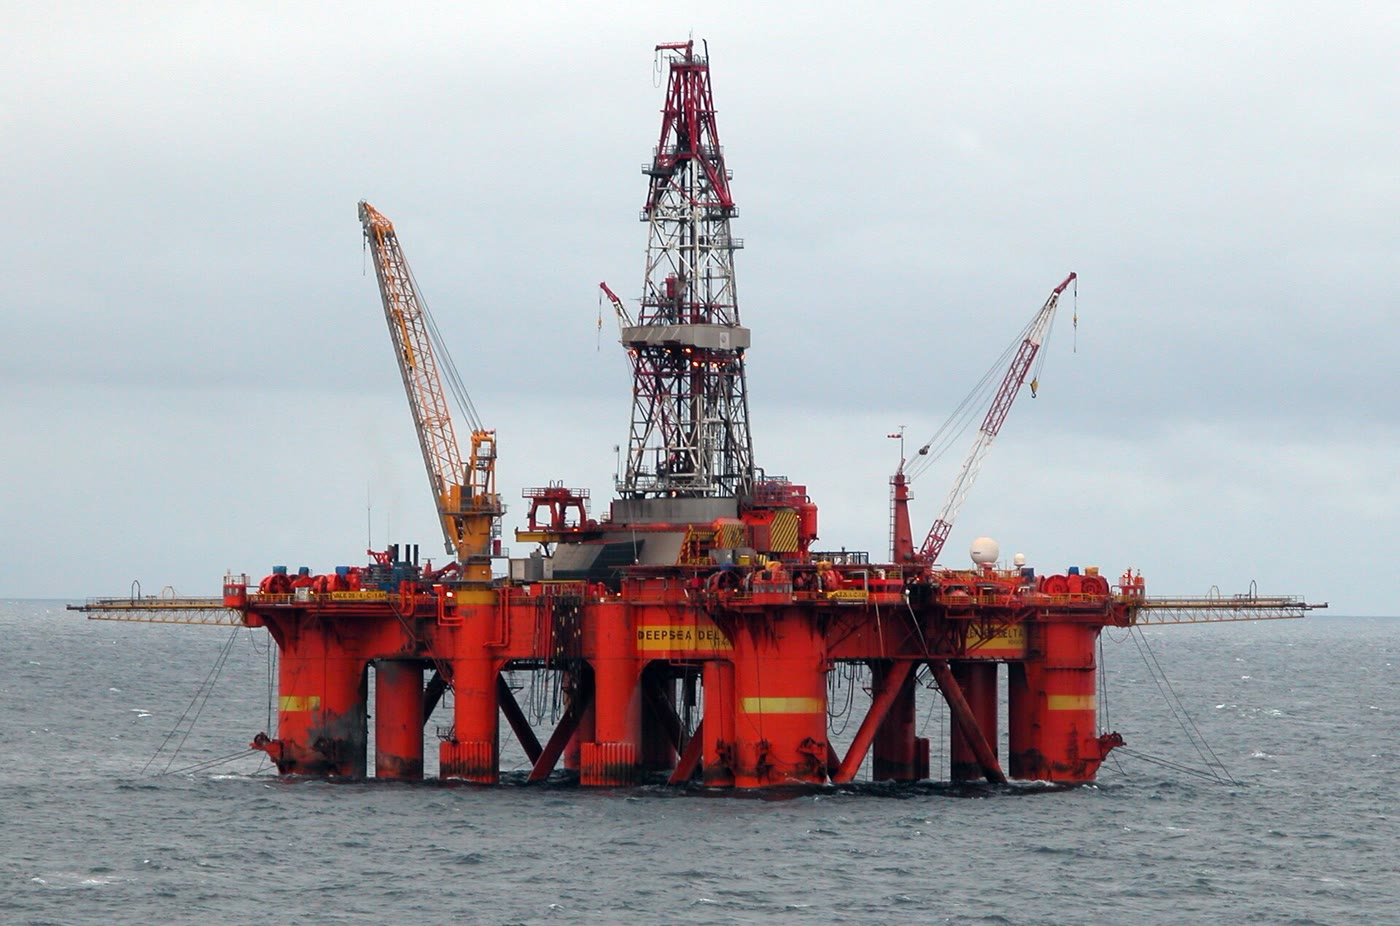
\includegraphics[width=0.66\linewidth]{images/book4/b2-16-drilling-rig.jpg}
\par\smallskip{\small उत्तरी सागर में एक अर्ध-निमज्जनीय वेधन-रिग। ऐसे रिगों से खोदे गए
बोरहोल वे मोटाइयाँ, आयु और शैल-प्रकार देते हैं जिनसे किसी द्रोणी के अवधसान का
पुनर्निर्माण होता है। फ़ोटो: Erik Christensen, 2005, CC BY-SA 3.0।}
\end{omfigure}

\section{द्रोणियाँ और उन्हें धँसाने वाले कारक}\label{sec:b2:basins-compared:types}

पुस्तक 3 ने द्रोणियों में उनकी स्थिति के आधार पर भेद किया था। यहाँ उनमें इस आधार पर भेद किया जाता है कि
उनके अवधसान को क्या चलाता है।

\begin{definition}[अंतःक्रेटॉनिक, दरार और निष्क्रिय-किनारा द्रोणियाँ]\label{def:b2:basins-compared:types}
\emph{अंतःक्रेटॉनिक द्रोणी}\index{अंतःक्रेटॉनिक द्रोणी} किसी महाद्वीप के भीतरी भाग में, प्लेट-सीमाओं से दूर,
एक चौड़ी, गोल या अंडाकार द्रोणी है, जो बड़े भ्रंशन के बिना बहुत लंबे समय तक धीरे-धीरे
धँसती है। \emph{दरार-द्रोणी}\index{दरार-द्रोणी} खिंचते हुए महाद्वीपीय स्थलमंडल में सामान्य भ्रंशों से
घिरी द्रोणी है; उसका अवधसान स्थलमंडल के खिंचाव और फिर
शीतलन का अनुसरण करता है। \emph{निष्क्रिय-किनारा द्रोणी}\index{निष्क्रिय-किनारा द्रोणी} अवसाद की वह
कील है, जो महासागर की ओर मोटी होती जाती है और विखंडन के बाद किसी महाद्वीपीय किनारे पर, पुरानी दरार की पतली हुई
भूपर्पटी के ऊपर, संचित होती है।
\end{definition}

\cref{ch:b2:alpine-orogen} की \omterm{def:b2:alpine-orogen:foreland}{अग्रभूमि द्रोणी} सूची पूरी करती है, और जो द्रोणियाँ
स्ट्राइक-स्लिप भ्रंशों के अनुदिश खुलती हैं वे पुस्तक 5 (स्नातक वर्ष 3) के लिए छोड़ी गई हैं। तीन क्रियाविधियाँ किसी
द्रोणी के तल को धँसाती हैं:
\begin{itemize}
  \item \emph{यांत्रिक} पतलापन: जब भूपर्पटी भ्रंशों द्वारा खींची और पतली की जाती है, हल्की
        भूपर्पटी का स्थान सघनतर प्रावार लेता है और समस्थिति बहाल करने के लिए सतह नीचे जाती है;
  \item \emph{तापीय} संकुचन: जो स्थलमंडल खिंचाव से या नीचे से गर्म हुआ हो, वह
        बाद में ठंडा होता है, सघनतर होता है और धँसता है, धीरे-धीरे, दसियों मिलियन वर्षों में;
  \item \emph{भारण}: किसी अधिक्षेप-पट्टी का, या स्वयं अवसाद का, भार
        स्थलमंडल को नीचे झुकाता है; वह आनमन पुस्तक 5 का विषय है, और यहाँ अवसाद-भार का
        स्थानीय, एयरी रूप पर्याप्त है।
\end{itemize}
\omterm{def:b2:basins-compared:types}{दरार-द्रोणियाँ} पहली दो को मिलाती हैं, निष्क्रिय किनारे दूसरी को अपने दरार-चरण से विरासत में पाते हैं,
\omterm{def:b2:alpine-orogen:foreland}{अग्रभूमि द्रोणियाँ} तीसरी से बनती हैं। \omterm{def:b2:basins-compared:types}{अंतःक्रेटॉनिक द्रोणियाँ} सबसे कम समझी गई हैं।

\begin{omfigure}
\centering
\begin{tikzpicture}[x=1cm, y=1cm, font=\scriptsize, line join=round,
  sed/.style={fill=yellow!35, draw=black!60, line width=0.3pt},
  crust/.style={fill=orange!25, draw=black!60, line width=0.3pt},
  mlith/.style={fill=green!12, draw=black!60, line width=0.3pt},
  asth/.style={fill=red!12, draw=black!60, line width=0.3pt},
  sea/.style={fill=blue!8, draw=none},
  ttl/.style={anchor=south west, font=\scriptsize\bfseries}]
% (a) intracratonic
\begin{scope}
\fill[asth] (0,-2.4) rectangle (6.6,-1.6);
\fill[mlith] (0,-1.6) rectangle (6.6,-0.7);
\fill[crust] (0,-0.7) -- (6.6,-0.7) -- (6.6,0) -- (4.9,0) .. controls (4.1,-0.45) and (2.5,-0.45) .. (1.7,0) -- (0,0) -- cycle;
\fill[sed] (1.7,0) .. controls (2.5,-0.45) and (4.1,-0.45) .. (4.9,0) -- cycle;
\draw[black!70] (0,0) -- (6.6,0);
\node[ttl] at (0,0.05) {(क) अंतःक्रेटॉनिक};
\node at (3.3,-1.15) {प्रावार-स्थलमंडल};
\node at (3.3,-2.0) {दुर्बलमंडल};
\end{scope}
% (b) rift
\begin{scope}[xshift=7.2cm]
\fill[asth] (0,-2.4) -- (6.6,-2.4) -- (6.6,-1.6) -- (4.5,-1.6) -- (3.3,-1.0) -- (2.1,-1.6) -- (0,-1.6) -- cycle;
\fill[mlith] (0,-1.6) -- (2.1,-1.6) -- (3.3,-1.0) -- (4.5,-1.6) -- (6.6,-1.6) -- (6.6,-0.7) -- (4.4,-0.7) -- (3.3,-0.45) -- (2.2,-0.7) -- (0,-0.7) -- cycle;
\fill[crust] (0,-0.7) -- (2.2,-0.7) -- (3.3,-0.45) -- (4.4,-0.7) -- (6.6,-0.7) -- (6.6,0) -- (4.6,0) -- (4.25,-0.42) -- (3.75,-0.2) -- (3.35,-0.4) -- (2.95,-0.15) -- (2.45,-0.42) -- (2.0,0) -- (0,0) -- cycle;
\fill[sed] (2.0,0) -- (2.45,-0.42) -- (2.95,-0.15) -- (3.35,-0.4) -- (3.75,-0.2) -- (4.25,-0.42) -- (4.6,0) -- cycle;
\draw[thick] (2.0,0) -- (2.5,-0.5) (4.6,0) -- (4.2,-0.5) (2.95,-0.15) -- (3.4,-0.48);
\draw[black!70] (0,0) -- (6.6,0);
\node[ttl] at (0,0.05) {(ख) दरार};
\node at (1.45,-1.15) {प्रावार-स्थलमंडल};
\node at (5.4,-2.0) {दुर्बलमंडल};
\end{scope}
% (c) passive margin
\begin{scope}[yshift=-3.3cm]
\fill[asth] (0,-2.4) -- (6.6,-2.4) -- (6.6,-1.2) -- (0,-1.6) -- cycle;
\fill[mlith] (0,-1.6) -- (6.6,-1.2) -- (6.6,-1.0) -- (4.2,-1.05) -- (2.4,-0.75) -- (0,-0.7) -- cycle;
\fill[crust] (0,-0.7) -- (2.4,-0.75) -- (4.2,-1.05) -- (4.2,-0.85) -- (2.6,-0.25) -- (1.6,0) -- (0,0) -- cycle;
\fill[gray!35, draw=black!60, line width=0.3pt] (4.2,-1.05) -- (6.6,-1.0) -- (6.6,-0.85) -- (4.2,-0.85) -- cycle;
\fill[sed] (1.6,0) -- (2.6,-0.25) -- (4.2,-0.85) -- (6.6,-0.85) -- (6.6,-0.55) -- (3.6,-0.45) -- (2.6,-0.05) -- (2.2,0) -- cycle;
\fill[sea] (2.2,0) -- (6.6,0) -- (6.6,-0.55) -- (3.6,-0.45) -- (2.6,-0.05) -- cycle;
\draw[black!70] (0,0) -- (2.2,0);
\draw[blue!60!black] (2.2,0) -- (6.6,0);
\node[ttl] at (0,0.05) {(ग) निष्क्रिय किनारा};
\node at (5.4,-0.95) {\tiny महासागरीय भूपर्पटी};
\node at (1.3,-2.0) {दुर्बलमंडल};
\node at (1.3,-1.05) {प्रावार-स्थलमंडल};
\end{scope}
% (d) foreland
\begin{scope}[xshift=7.2cm, yshift=-3.3cm]
\fill[asth] (0,-2.4) -- (6.6,-2.4) -- (6.6,-2.0) -- (0,-1.5) -- cycle;
\fill[mlith] (0,-1.5) -- (6.6,-2.0) -- (6.6,-1.2) -- (0,-0.7) -- cycle;
\fill[crust] (0,-0.7) -- (6.6,-1.2) -- (6.6,-0.55) -- (3.6,-0.4) .. controls (2.0,-0.15) .. (0,0) -- cycle;
\fill[sed] (0,0) .. controls (2.0,-0.15) .. (3.6,-0.4) -- (6.6,-0.55) -- (5.0,0) -- cycle;
\fill[crust, fill=orange!45] (5.0,0) -- (6.6,-0.55) -- (6.6,0.6) -- (6.1,0.6) -- cycle;
\draw[thrust fault] (6.6,-0.55) -- (5.0,0);
\draw[black!70] (0,0) -- (5.0,0);
\node[ttl] at (0,0.05) {(घ) अग्रभूमि};
\node[anchor=north east, font=\tiny] at (6.55,0.55) {पट्टी};
\node at (2.2,-1.25) {प्रावार-स्थलमंडल};
\node at (1.5,-2.05) {दुर्बलमंडल};
\end{scope}
\end{tikzpicture}
\par\smallskip{\small स्थलमंडल के आर-पार योजनामूलक काटों में द्रोणियों के चार परिवार (पैमाने के
बिना; अवसाद पीला, महाद्वीपीय भूपर्पटी नारंगी, महासागरीय भूपर्पटी धूसर)। ऊर्ध्वाधर
अतिशयोक्ति बड़ी है: वास्तविक द्रोणियाँ सैकड़ों किलोमीटर चौड़ी और कुछ से पंद्रह
किलोमीटर तक गहरी होती हैं।}
\end{omfigure}

उत्तरी सागर की \omterm{def:b2:basins-compared:types}{दरार-द्रोणियाँ} पहली दो क्रियाविधियों का क्लासिकी उदाहरण हैं। वहाँ ट्राइऐसिक से
ग्राबेन बने, और अंतिम बड़ा खिंचाव मध्य जुरैसिक से
मध्य-क्रिटेशस तक चला; फिर भ्रंश शांत हो गए, और द्रोणी का मध्य भाग एक चौड़ी तश्तरी के रूप में
धँसता रहा, जिसे चॉक, बलुआ पत्थर और, अधिकांश टर्शियरी के दौरान, शेल और
पंकाश्म भरते गए। केवल जल से भारित होने पर, भ्रंशन रुकने के बाद उसका आधारशैल मध्य में 1100 से
\qty{1400}{m} और पार्श्वों पर 600 से \qty{700}{m} और धँसा होता।
% ledger: sc80b4:north-sea

पूर्वी संयुक्त राज्य अमेरिका का निष्क्रिय किनारा वही अवधसान बड़े पैमाने पर दिखाता है।
शेल्फ़ के आर-पार भूकंपीय प्रोफ़ाइल बाल्टीमोर कैन्यन द्रोणी में मेसोज़ोइक और उससे नई चट्टान की \qty{14}{km} से अधिक
और जॉर्जेस बैंक द्रोणी में \qty{8}{km} मोटाई दिखाते हैं, ऐसी इकाइयों में जो महासागर की ओर
मोटी होती जाती हैं। उसके जुरैसिक निक्षेप-केंद्र दरार की संरचनाओं और उसके
बाद के तापीय अवधसान के मंडलों का अनुसरण करते हैं।
% ledger: schlee76:atlantic, lang24:atlantic

मिशिगन द्रोणी \omterm{def:b2:basins-compared:types}{अंतःक्रेटॉनिक द्रोणियों} का प्रतिरूप है। अंडाकार, कुछ लाख
वर्ग किलोमीटर क्षेत्रफल वाली, इसमें कोई 500 मिलियन वर्षों में अलग-अलग प्रकरणों में जमा \qty{4}{km} से अधिक
फ़ैनेरोज़ोइक अवसाद है, बहुत कम भ्रंशन के साथ। इसके तेज़
अवधसान के प्रकरण उत्तर अमेरिका और अन्य महाद्वीपों के भीतरी भागों की अन्य द्रोणियों के प्रकरणों से संपाती हैं,
जो किसी एक द्रोणी से बड़े कारण का संकेत देता है। 57\,000 से अधिक
कूप-लॉगों का \omterm{def:b2:basins-compared:backstripping}{बैकस्ट्रिपिंग} अवधसान का एक दीर्घजीवी, लगभग वृत्ताकार प्रतिरूप दिखाता है, जिसके बारे में लेखक सुझाते हैं कि
प्रावार का अधोप्रवाह उसकी व्याख्या कर सकता है, और जो महाद्वीप के दूर के किनारे पर दो पर्वतजननों के समय
बाधित हुआ। \omterm{def:b2:basins-compared:types}{अंतःक्रेटॉनिक द्रोणियाँ} क्यों धँसती हैं, इस पर अब भी बहस है।
% ledger: sloss82:michigan, crowe09:michigan

\section{अवधसान वक्र}\label{sec:b2:basins-compared:curves}

एक कुआँ, या एक मापी गई काट, हर इकाई के लिए उसकी वर्तमान गहराई, उसका शैल-प्रकार और उसकी आयु देता है,
जो जीवाश्मों से या सहसंबंध से पढ़ी जाती है। जल की उस गहराई के साथ जिसमें हर इकाई जमी थी,
जो उसके जीवाश्मों और अवसादी संरचनाओं से पढ़ी जाती है, यह द्रोणी का इतिहास देता है।

\begin{definition}[अवधसान वक्र]\label{def:b2:basins-compared:curve}
किसी स्थल पर किसी द्रोणी का \emph{अवधसान वक्र}\index{अवधसान वक्र} किसी संदर्भ-सतह की, प्रायः
आधारशैल या सबसे पुरानी इकाई के आधार की, समुद्र-तल के नीचे गहराई का
समय के विरुद्ध आलेख है। \emph{कुल} अवधसान वक्र हर समय पर जैसी थी वैसी अवसाद-मोटाई,
और जल की गहराई, का उपयोग करता है; \emph{विवर्तनिक} अवधसान वक्र अवसाद के स्थान पर जल रखता है
और उसका समस्थितिक प्रभाव हटा देता है।
\end{definition}

कोई इकाई अतीत में कभी उतनी मोटी नहीं होती जितनी आज है। दबने पर उसकी छिद्रता घटी; उसके कण
नहीं बदले, पर उसका जल निचोड़ दिया गया। पुस्तक 3 ने गहराई
$z$ पर छिद्रता को एथी के नियम के रूप में लिखा, $\phi(z) = \phi_0\,e^{-z/c}$, और
$z_1$ और $z_2$ के बीच की किसी परत की ठोस मोटाई निकाली,
\[
  T_s = (z_2 - z_1) - \phi_0 c\left(e^{-z_1/c} - e^{-z_2/c}\right),
\]
जो परत के खिसकने पर वही रहती है। किसी इकाई को उथली स्थिति तक \emph{डिकंपैक्ट} करने के लिए,
जिसका शीर्ष अब $z_1'$ पर हो, वह आधार $z_2'$ खोजा जाता है जो वही ठोस मोटाई रखे।
इस समीकरण का कोई संवृत हल नहीं है, पर नियत-बिंदु पुनरावृत्ति
\[
  z_2' \leftarrow z_1' + T_s + \phi_0 c\left(e^{-z_1'/c} - e^{-z_2'/c}\right)
\]
जो $z_2' = z_1' + T_s$ से आरंभ होती है, कुछ ही चरणों में अभिसरित हो जाती है। परत का प्रति इकाई क्षेत्रफल द्रव्यमान
उसके कणों के द्रव्यमान और उसके छिद्र-जल के द्रव्यमान का योग है,
\[
  m = \rho_g T_s + \rho_w\,(z_2 - z_1 - T_s),
\]
जहाँ $\rho_g$ कणों का घनत्व है; किसी स्तंभ के द्रव्यमान को उसकी मोटाई से भाग देने पर
उसका माध्य घनत्व $\bar\rho_s$ मिलता है।

इस अध्याय में प्रयुक्त शैल-प्रकारों, यानी रेत, शेल, चॉक और शेलयुक्त रेत, के लिए नीचे की तालिका
स्क्लेटर और क्रिस्टी (1980) के स्थिरांक देती है, जैसे वे एक मुक्त-स्रोत प्रोग्राम में संकलित हैं।
रेत अपनी छिद्रता सबसे गहराई तक बनाए रखती है, चॉक उसे सबसे तेज़ी से खोता है।
% ledger: pybacktrack:compaction

\begin{center}
\small
\begin{tabular}{lccc}
\hline
शैल-प्रकार & कण-घनत्व (\unit{kg.m^{-3}}) & सतही छिद्रता $\phi_0$ & क्षय-लंबाई $c$ (\unit{m}) \\
\hline
रेत & 2650 & 0.49 & 3704 \\
शेल & 2700 & 0.63 & 1960 \\
चॉक & 2710 & 0.70 & 1408 \\
शेलयुक्त रेत & 2680 & 0.56 & 2564 \\
\hline
\end{tabular}
\end{center}

\section{बैकस्ट्रिपिंग}\label{sec:b2:basins-compared:backstripping}

कुल \omterm{def:b2:basins-compared:curve}{अवधसान वक्र} दो कारणों को मिलाता है: जिसने भी द्रोणी बनाई, और उसका भार जिसने उसे
भरा। उन्हें अलग करना अगली प्रक्रिया का उद्देश्य है, जो द्रोणी-विश्लेषण का
केंद्रीय उपकरण है।

\begin{definition}[बैकस्ट्रिपिंग]\label{def:b2:basins-compared:backstripping}
\emph{बैकस्ट्रिपिंग}\index{बैकस्ट्रिपिंग} किसी द्रोणी के समय के साथ विवर्तनिक अवधसान का
पुनर्निर्माण है: किसी कुएँ की इकाइयाँ एक-एक करके, सबसे नई से आरंभ करके, हटाई जाती हैं,
हर चरण पर शेष इकाइयाँ डिकंपैक्ट की जाती हैं, और अवसाद और जल के
भार का समस्थितिक प्रभाव हटाकर वह गहराई निकाली जाती है जिस पर आधारशैल केवल जल के नीचे खड़ा होता।
\end{definition}

अंतिम चरण एक समस्थितिक संतुलन है। पुस्तक 3 ने इसे समुद्र-तल तक भरी द्रोणी के लिए बनाया था;
सामान्य स्थिति में जल की गहराई और समुद्र का स्तर जुड़ जाते हैं।

\begin{proposition}[एयरी बैकस्ट्रिपिंग]\label{prop:b2:basins-compared:backstrip}
मान लीजिए किसी समय कोई द्रोणी मोटाई $S$ और माध्य घनत्व
$\bar\rho_s$ का अवसाद-स्तंभ रखती है, जल की गहराई $W_d$ के नीचे, जबकि समुद्र अपने वर्तमान स्तर से
$\Delta_{SL}$ ऊपर था। घनत्व $\rho_m$ के प्रावार पर स्थानीय समस्थिति में, घनत्व $\rho_w$ के जल के साथ,
उस समय का विवर्तनिक अवधसान, वर्तमान समुद्र-तल से मापा गया, है
\[
  Y = S\,\frac{\rho_m - \bar\rho_s}{\rho_m - \rho_w} + W_d
      - \Delta_{SL}\,\frac{\rho_m}{\rho_m - \rho_w}.
\]
\end{proposition}

\begin{proof}
दोनों के नीचे एक प्रतिपूर्ति-गहराई तक, एक ही स्थलमंडल के ऊपर दो स्तंभों की तुलना कीजिए।
पहले में गहराई $W_d$ का जल मोटाई $S$ के अवसाद के ऊपर है; दूसरे में केवल जल
उसी समुद्र-सतह के नीचे गहराई $Y'$ की एक द्रोणी भरता है। उनके द्रव्यमान बराबर हैं:
\[
  \rho_w W_d + \bar\rho_s S + \rho_m\,(d - W_d - S) = \rho_w Y' + \rho_m\,(d - Y'),
\]
जहाँ $d$ समुद्र-सतह के नीचे प्रतिपूर्ति-स्तर की साझा गहराई है। अतः
$Y'(\rho_m - \rho_w) = S(\rho_m - \bar\rho_s) + W_d(\rho_m - \rho_w)$, जो पहले दो
पद हैं। यदि समुद्र आज से $\Delta_{SL}$ ऊँचा था, तो वह अतिरिक्त जल द्रोणी के
अपने अवधसान का भाग नहीं है: उसे हटाने पर जल-भारित आधारशैल
$\Delta_{SL}\rho_w/(\rho_m - \rho_w)$ ऊपर उठता है, और आज के समुद्र-तल के नीचे उसकी गहराई फिर
$\Delta_{SL}$ कम हो जाती है; दोनों मिलाकर, $\Delta_{SL}\,\rho_m/(\rho_m - \rho_w)$।
\end{proof}
% ledger: pybacktrack:backstrip

$\rho_m = \qty{3330}{kg.m^{-3}}$ और $\rho_w = \qty{1030}{kg.m^{-3}}$ के साथ,
\qty{2300}{kg.m^{-3}} माध्य घनत्व का अवसाद-स्तंभ विवर्तनिक अवधसान में अपनी मोटाई के $1030/2300 = 0.45$ के बराबर
गिना जाता है: किसी द्रोणी के भराव की आधी से अधिक मोटाई के लिए जगह उसका अपना भार बनाता है।
आज से \qty{100}{m} ऊँचा समुद्र परिणाम को \qty{145}{m} घटा देता है। जल की गहराई और
अतीत का समुद्र-स्तर सबसे दुर्बल आँकड़े हैं: जीवाश्म जल-गहराइयों का एक परास देते हैं, जो ढलान पर प्रायः सैकड़ों
मीटर चौड़ा होता है, और विवर्तनिक अवधसान वह परास विरासत में पाता है।

\begin{method}[किसी कुएँ का बैकस्ट्रिपिंग]\label{met:b2:basins-compared:backstrip}
\begin{enumerate}
  \item आधार से आरंभ करके इकाइयों की सूची बनाइए: उनके शीर्षों और आधारों की वर्तमान गहराइयाँ, उनके
        शैल-प्रकार के स्थिरांक $(\rho_g, \phi_0, c)$, उनके शीर्षों की आयु, और उनमें से हर आयु पर
        जल की गहराई।
  \item हर इकाई की ठोस मोटाई $T_s$ उसकी वर्तमान गहराइयों से निकालिए।
  \item इकाई $k$ के शीर्ष की आयु के लिए, सभी नई इकाइयाँ हटाइए। इकाई $k$ का शीर्ष
        शून्य गहराई पर रखकर उसे डिकंपैक्ट कीजिए; फिर हर पुरानी इकाई को, बारी-बारी से, अपने ऊपर वाली के नीचे रखकर
        डिकंपैक्ट कीजिए।
  \item मोटाइयों को जोड़कर $S$ पाइए, और द्रव्यमानों को जोड़कर माध्य घनत्व
        $\bar\rho_s = \sum m / S$।
  \item $Y$ पाने के लिए \cref{prop:b2:basins-compared:backstrip} लागू कीजिए; कुल अवधसान
        $S + W_d$ है।
  \item हर आयु के लिए, सबसे पुरानी से वर्तमान तक, दोहराइए; $Y$ और $S + W_d$ को आयु के विरुद्ध आलेखित कीजिए।
\end{enumerate}
\end{method}

नीचे का चित्र एक \omterm{def:b2:basins-compared:types}{दरार-द्रोणी} के एक कल्पित कुएँ का परिणाम दिखाता है। चार इकाइयों के कोर लिए गए:
दरार-कालीन रेत, जो भ्रंशों के सक्रिय रहते 165 और \qty{150}{Ma} के बीच जमी; फिर शेल,
चॉक और शेलयुक्त रेत। आज कोई डिकंपैक्शन आवश्यक नहीं: आधारशैल \qty{6030}{m} पर है
और स्तंभ का माध्य घनत्व \qty{2358}{kg.m^{-3}} है, अतः $Y = \qty{2648}{m}$,
\qty{100}{m} जल के नीचे। \qty{150}{Ma} पर, अकेली रेत, सतह पर डिकंपैक्ट करने पर,
\qty{2239}{m} मोटी थी, माध्य घनत्व \qty{2055}{kg.m^{-3}} के साथ:
\qty{200}{m} जल के नीचे, $Y = \qty{1441}{m}$। कुल अवधसान
विवर्तनिक अवधसान के दुगुने से अधिक है, और विवर्तनिक वक्र एक तेज़ पहला चरण, फिर
मंद होता धँसाव दिखाता है: एक दरार का आकार।
% values (script): figdata/bachelor-2/basins.py part numbers (S_150 2239.5, rho_0 2357.9, Y_0 2648.7, Y_150 1442.1); printed from the rounded chain of calc/ch16.py (rho 2358 -> 2648; T 2239, rho 2055 -> 1441), as in the problem

\begin{omfigure}
\centering
% figdata/bachelor-2/basins.py parts stages and fit (invented well)
\begin{tikzpicture}
\begin{axis}[width=0.8\linewidth, height=6.0cm, x dir=reverse, y dir=reverse, xmin=0, xmax=170,
  ymin=0, ymax=6500, xlabel={आयु (\unit{Ma})}, ylabel={समुद्र-तल के नीचे गहराई (\unit{m})},
  tick label style={font=\scriptsize}, label style={font=\small}, xtick={0,25,...,175},
  xtick pos=bottom, ytick pos=left,
  legend style={at={(0.5,1.04)}, anchor=south, draw=none, font=\scriptsize, legend columns=3,
  /tikz/every even column/.append style={column sep=8pt}}]
\addplot[omThm, line width=1pt, mark=*, mark size=1.6pt] table[x=age_Ma, y=total_m]
  {figdata/out/bachelor-2-basins-stages.dat};
\addlegendentry{कुल अवधसान $S + W_d$}
\addplot[blue!70!black, line width=1pt, mark=square*, mark size=1.6pt] table[x=age_Ma, y=Y_m]
  {figdata/out/bachelor-2-basins-stages.dat};
\addlegendentry{विवर्तनिक अवधसान $Y$}
\addplot[black!70, dashed, line width=0.8pt] table[x=age_Ma, y=Y_m]
  {figdata/out/bachelor-2-basins-fit.dat};
\addlegendentry{खिंचाव प्रतिरूप, $\beta = 1.50$}
\node[font=\scriptsize, anchor=south west] at (axis cs:149,1500) {दरार-चरण का अंत};
\end{axis}
\end{tikzpicture}
\par\smallskip{\small चार इकाइयों वाले एक कल्पित कुएँ का \omterm{def:b2:basins-compared:backstripping}{बैकस्ट्रिपिंग} (आँकड़े सप्ताहांत
समस्या में): हर समय पर जैसा था वैसे अवसाद के साथ आधारशैल की गहराई, और विवर्तनिक अवधसान,
दरार-चरण के अंत के अवधसान से मिलाए गए \omterm{def:b2:basins-compared:stretching}{खिंचाव प्रतिरूप} के वक्र के साथ
(\cref{sec:b2:basins-compared:stretching})।}
\end{omfigure}

\begin{omfigure}
\centering
\begin{tikzpicture}[x=1cm, y=0.1cm, font=\scriptsize, line join=round,
  u/.style={draw=black!60, line width=0.3pt}]
% today
\begin{scope}
\fill[blue!8] (0,0) rectangle (1.6,-1.0);
\fill[u, fill=yellow!25] (0,-1.0) rectangle (1.6,-18.0);
\fill[u, fill=green!18] (0,-18.0) rectangle (1.6,-34.1);
\fill[u, fill=gray!25] (0,-34.1) rectangle (1.6,-45.2);
\fill[u, fill=yellow!55] (0,-45.2) rectangle (1.6,-61.3);
\draw[black!70] (0,-61.3) -- (1.6,-61.3);
\node[anchor=south] at (0.8,0.1) {आज};
\node at (0.8,-9.5) {शेलयुक्त रेत};
\node at (0.8,-26) {चॉक};
\node at (0.8,-39.6) {शेल};
\node at (0.8,-53.2) {रेत};
\node[anchor=north] at (0.8,-61.5) {\qty{6130}{m}};
\end{scope}
% at 150 Ma
\begin{scope}[xshift=3.0cm]
\fill[blue!8] (0,0) rectangle (1.6,-2.0);
\fill[u, fill=yellow!55] (0,-2.0) rectangle (1.6,-24.39);
\draw[black!70] (0,-24.4) -- (1.6,-24.4);
\node[anchor=south] at (0.8,0.1) {\qty{150}{Ma}};
\node at (0.8,-13.2) {रेत};
\node[anchor=north] at (0.8,-24.6) {\qty{2439}{m}};
\end{scope}
\draw[-{Latex}, thick] (4.9,-12) -- (6.1,-12) node[midway, above] {भार हटाएँ};
% water loaded
\begin{scope}[xshift=6.3cm]
\fill[blue!20] (0,0) rectangle (1.6,-14.4);
\draw[black!70] (0,-14.4) -- (1.6,-14.4);
\node[anchor=south] at (0.8,0.1) {केवल जल};
\node at (0.8,-7.2) {जल};
\node[anchor=north] at (0.8,-14.6) {$Y = \qty{1441}{m}$};
\end{scope}
\draw[black!40, dashed] (-0.3,0) -- (8.2,0);
\node[anchor=west] at (8.2,0) {समुद्र-तल};
\end{tikzpicture}
\par\smallskip{\small \qty{150}{Ma} पर कल्पित कुएँ का \omterm{def:b2:basins-compared:backstripping}{बैकस्ट्रिपिंग} (गहराइयाँ पैमाने पर):
आज की चार इकाइयाँ; दरार-चरण के अंत पर अकेली रेत, सतह पर डिकंपैक्ट की हुई,
\qty{200}{m} जल के नीचे; केवल जल से भारित वही स्थलमंडल, जिसका आधारशैल
ऊँचा खड़ा है क्योंकि जल अवसाद से हल्का है।}
\end{omfigure}

\section{खिंचाव प्रतिरूप}\label{sec:b2:basins-compared:stretching}

कोई \omterm{def:b2:basins-compared:types}{दरार-द्रोणी} पहले तेज़ी से और फिर धीरे-धीरे क्यों धँसती है? 1978 में डी॰ मैकेंज़ी ने एक ऐसा प्रतिरूप प्रस्तावित किया
जो इतना सरल है कि उसके प्राचलों को एक ही कुएँ से मिलाया जा सकता है।

\begin{definition}[खिंचाव प्रतिरूप; खिंचाव-गुणक; दरार-कालीन और दरार-उत्तर अवधसान]\label{def:b2:basins-compared:stretching}
किसी द्रोणी का \emph{खिंचाव प्रतिरूप}\index{खिंचाव प्रतिरूप} दरार-निर्माण को समूचे स्थलमंडल के
शुद्ध अपरूपण द्वारा तात्क्षणिक, एकसमान खिंचाव के रूप में दर्शाता है: भूपर्पटी और प्रावार-स्थलमंडल
एक ही गुणक से पतले होते हैं, और गर्म दुर्बलमंडल निष्क्रिय रूप से ऊपर उठकर
जगह भरता है, जिसके बाद स्थलमंडल ठंडा होता है। \emph{खिंचाव-गुणक}\index{खिंचाव-गुणक}
$\beta$ खिंचे हुए क्षेत्र की खिंचाव के बाद की चौड़ाई और उसके पहले की चौड़ाई का अनुपात है,
जो भूपर्पटी की प्रारंभिक और अंतिम मोटाई के अनुपात के बराबर है। खिंचाव के
दौरान उत्पन्न अवधसान \emph{दरार-कालीन अवधसान}\index{दरार-कालीन अवधसान} है; जो
बाद में स्थलमंडल के शीतलन से उत्पन्न होता है वह \emph{दरार-उत्तर
अवधसान}\index{दरार-उत्तर अवधसान}, या तापीय अवधसान, है।
\end{definition}

प्रकृति में खिंचाव एक परिमित समय लेता है, मिलियनों वर्ष। प्रतिरूप के बाद के संस्करण उसे
चलने देते हैं, पर जब तक वह बहुत धीमा न हो, सरल तात्क्षणिक संस्करण अवधसान को
मोटे तौर पर, किंतु सही, देता है, क्योंकि खिंचाव के बाद शीतलन लगभग उसी तरह चलता है।
% ledger: sheplev98:model

\begin{omfigure}
\centering
\begin{tikzpicture}[x=0.5cm, y=0.5cm, font=\scriptsize, line join=round]
% before
\begin{scope}
\fill[orange!25, draw=black!60, line width=0.3pt] (0,0) rectangle (4,-2.8);
\fill[green!12, draw=black!60, line width=0.3pt] (0,-2.8) rectangle (4,-10);
\fill[red!12, draw=black!60, line width=0.3pt] (0,-10) rectangle (4,-11.5);
\node at (2,-1.4) {भूपर्पटी $t_c$};
\node[align=center] at (2,-6.4) {प्रावार-\\स्थलमंडल};
\node at (2,-10.75) {दुर्बलमंडल};
\draw[|-|] (-0.4,0) -- (-0.4,-10) node[midway, left] {$a$};
\node[anchor=south] at (2,0.2) {पहले: चौड़ाई $\ell$};
\node[anchor=north] at (2,-11.6) {तापमान $0$ से $T_1$};
\end{scope}
% after
\begin{scope}[xshift=4.6cm]
\fill[blue!20] (0,0) rectangle (8,-1.0);
\fill[orange!25, draw=black!60, line width=0.3pt] (0,-1.0) rectangle (8,-2.4);
\fill[green!12, draw=black!60, line width=0.3pt] (0,-2.4) rectangle (8,-6.0);
\fill[red!12, draw=black!60, line width=0.3pt] (0,-6.0) rectangle (8,-11.5);
\draw[black!60, dashed] (0,-10) -- (8,-10);
\node at (4,-0.5) {जल, गहराई $S_i$};
\node at (4,-1.7) {भूपर्पटी $t_c/\beta$};
\node at (4,-4.2) {प्रावार-स्थलमंडल $a/\beta$};
\node[align=center] at (4,-8.0) {$T_1$ पर दुर्बलमंडल,\\निष्क्रिय रूप से उठा};
\node[anchor=south west] at (0,-10) {स्थलमंडल का पुराना आधार};
\node[anchor=south] at (4,0.2) {खिंचाव के ठीक बाद: चौड़ाई $\beta\ell$};
\node[anchor=north] at (4,-11.6) {फिर वह ठंडा होता, मोटा होता और धँसता है};
\draw[black!40] (0,0) -- (8,0);
\end{scope}
\end{tikzpicture}
\par\smallskip{\small \omterm{def:b2:basins-compared:stretching}{खिंचाव प्रतिरूप} (पैमाने के बिना): मोटाई $a$ का, भूपर्पटी
$t_c$ वाला स्थलमंडल अपनी चौड़ाई के $\beta$ गुना तक खींचा जाता है; भूपर्पटी और प्रावार-स्थलमंडल
$\beta$ से पतले होते हैं, दुर्बलमंडल ऊपर उठता है, और सतह जल के नीचे \omterm{def:b2:basins-compared:stretching}{दरार-कालीन अवधसान} $S_i$ से
धँसती है। यहाँ $\beta = 2$।}
\end{omfigure}

\begin{proposition}[खिंचाव प्रतिरूप में अवधसान]\label{prop:b2:basins-compared:stretching}
मान लीजिए मोटाई $a$ के एक स्थलमंडल में, मोटाई $t_c$ की भूपर्पटी के साथ, एक रैखिक जियोथर्म है, जो
सतह पर $0$ से उसके आधार पर दुर्बलमंडल के तापमान $T_1$ तक जाता है; भूपर्पटी और प्रावार के
घनत्व $\rho_c(1 - \alpha T)$ और $\rho_m(1 - \alpha T)$ हों, जहाँ $\alpha$ तापीय
प्रसार-गुणांक है। यदि उसे $\beta$ से तात्क्षणिक रूप से खींचा जाए और द्रोणी को
घनत्व $\rho_w$ के जल से भरा जाए:
\begin{enumerate}
  \item \omterm{def:b2:basins-compared:stretching}{दरार-कालीन अवधसान} है
  \[
    S_i = \frac{a\left(1 - \dfrac{1}{\beta}\right)\left[(\rho_m - \rho_c)\dfrac{t_c}{a}
          \left(1 - \dfrac{\alpha T_1 t_c}{2a}\right) - \dfrac{\alpha T_1 \rho_m}{2}\right]}
          {\rho_m(1 - \alpha T_1) - \rho_w};
  \]
  \item खिंचाव के समय $t$ बाद \omterm{def:b2:basins-compared:stretching}{दरार-उत्तर अवधसान}, किसी श्रेणी के पहले पद तक, है
  \[
    S_t = E_0\,\frac{\beta}{\pi}\sin\frac{\pi}{\beta}\left(1 - e^{-t/\tau}\right),\qquad
    E_0 = \frac{4a\rho_m\alpha T_1}{\pi^2(\rho_m - \rho_w)},\qquad
    \tau = \frac{a^2}{\pi^2\kappa},
  \]
  जहाँ $\kappa$ तापीय विसरणशीलता है और $\tau$ स्थलमंडल का \emph{तापीय समय-स्थिरांक}\index{तापीय समय-स्थिरांक}
  है।
\end{enumerate}
\end{proposition}
% ledger: pybacktrack:rifting

\begin{proof}
(1) खिंचाव से पहले के स्तंभ की तुलना ठीक बाद के स्तंभ से कीजिए, स्थलमंडल के पुराने आधार तक,
जो खिंचाव से पहले सतह के नीचे गहराई $a$ पर है। पहले, मोटाई $t_c$ की भूपर्पटी
और प्रावार-स्थलमंडल तापमानों $T = T_1 z/a$ पर हैं; बाद में, दोनों
$\beta$ से पतले हैं और उनके तापमान $0$ से $T_1$ तक, $a/\beta$ के भीतर, चलते हैं, अतः जल के आधार के नीचे गहराई $z'$ पर
किसी बिंदु का $T = T_1\beta z'/a$ है; नीचे, $T_1$ पर दुर्बलमंडल का
घनत्व $\rho_m(1 - \alpha T_1)$ है; ऊपर, जल गहराई $S_i$ भरता है। घनत्व $\rho(1 - \alpha T)$ की
किसी परत का द्रव्यमान, जिसमें $T$ रैखिक रूप से $T_a$ से $T_b$ तक बढ़ता है,
$\rho\,h\,(1 - \alpha(T_a + T_b)/2)$ है। पहले, स्तंभ में है
\[
  \rho_c t_c\left(1 - \frac{\alpha T_1 t_c}{2a}\right)
  + \rho_m (a - t_c)\left(1 - \frac{\alpha T_1 (a + t_c)}{2a}\right);
\]
बाद में, उसमें जल, पतली हुई भूपर्पटी और प्रावार-स्थलमंडल, और वह दुर्बलमंडल है जो
गहराई $a$ का शेष भाग भरता है:
\[
  \rho_w S_i + \frac{\rho_c t_c}{\beta}\left(1 - \frac{\alpha T_1 t_c}{2a}\right)
  + \frac{\rho_m (a - t_c)}{\beta}\left(1 - \frac{\alpha T_1 (a + t_c)}{2a}\right)
  + \rho_m(1 - \alpha T_1)\left(a - S_i - \frac{a}{\beta}\right).
\]
समस्थिति दोनों को बराबर करती है। $S_i$ वाले पदों को एक ओर और गुणक
$(1 - 1/\beta)$ को दूसरी ओर इकट्ठा करके, और विस्तार करके, सूत्र मिलता है; बीजगणित
\cref{exo:b2:basins-compared:11} है।

(2) खिंचाव के बाद, प्लेट $0$ पर रखी सतह और $T_1$ पर रखे आधार के बीच चालन से ठंडी होती है,
उस रैखिक प्रोफ़ाइल की ओर जिससे वह चली थी। अतिरिक्त तापमान ऊष्मा-समीकरण को
शीर्ष और आधार पर शून्य मानों के साथ हल करता है, और इसलिए पदों
$b_n\sin(n\pi z/a)\,e^{-n^2\kappa\pi^2 t/a^2}$ का योग है; हर पद अपने समय, $\tau/n^2$, से ठंडा होता है।
खोई हुई ऊष्मा स्तंभ को $\alpha\int \Delta T\,\mathrm{d}z$ से सिकोड़ती है, और जगह भरने वाला अतिरिक्त
जल उसे गुणक $\rho_m/(\rho_m - \rho_w)$ से और धँसाता है। केवल विषम पद
योगदान करते हैं; पहला पद रखने पर, जिसका गुणांक प्रारंभिक प्रोफ़ाइल से निकाला जाता है,
व्यंजक मिलता है। शेष पद नौ या अधिक गुना तेज़ी से ठंडे होते हैं, और लगभग दस मिलियन वर्षों के बाद
वे अवधसान को लगभग नियत मात्रा से खिसकाते हैं, \qty{100}{m} से कम, नीचे के मानों के साथ $\beta$ के
1.2 से 4 तक के लिए।
\end{proof}
% values (script): basins.thermal_series vs basins.thermal, tested in tests/bachelor-2/test_basins.py

मैकेंज़ी के शोधपत्र के प्राचल हैं $a = \qty{125}{km}$, $T_1 = \qty{1333}{\celsius}$,
$\alpha = \qty{3.28e-5}{K^{-1}}$, $\kappa = \qty{8e-7}{m^2.s^{-1}}$, $\rho_m =
\qty{3330}{kg.m^{-3}}$ (\qty{0}{\celsius} पर), $\rho_c = \qty{2800}{kg.m^{-3}}$; \qty{1030}{kg.m^{-3}}
के समुद्री जल के साथ वे $\tau = \qty{62.7}{Myr}$ और $E_0 = \qty{3207}{m}$ देते हैं। \qty{35}{km} की
भूपर्पटी के साथ, \omterm{def:b2:basins-compared:stretching}{दरार-कालीन अवधसान} $S_i = \qty{4334}{m} \times (1 - 1/\beta)$ है।
% ledger: sheplev98:parameters, pybacktrack:rifting
% values (script): tau_Myr 62.7, E0_m 3206.9, Si_max_m 4333.8

\begin{omfigure}
\centering
% figdata/bachelor-2/basins.py part curves
\begin{tikzpicture}
\begin{axis}[width=0.8\linewidth, height=6.2cm, y dir=reverse, xmin=0, xmax=200, ymin=0,
  ymax=6500, xlabel={खिंचाव के बाद का समय (\unit{Myr})},
  ylabel={विवर्तनिक अवधसान (\unit{m})}, tick label style={font=\scriptsize},
  label style={font=\small}, xtick pos=bottom, ytick pos=left]
\addplot[black!45, line width=1pt] table[x=t_Myr, y=b1.2] {figdata/out/bachelor-2-basins-curves.dat};
\addplot[blue!70!black, line width=1pt] table[x=t_Myr, y=b1.5] {figdata/out/bachelor-2-basins-curves.dat};
\addplot[omThm, line width=1pt] table[x=t_Myr, y=b2] {figdata/out/bachelor-2-basins-curves.dat};
\addplot[orange!80!black, line width=1pt] table[x=t_Myr, y=b4] {figdata/out/bachelor-2-basins-curves.dat};
\node[font=\scriptsize, anchor=south west, inner sep=1pt] at (axis cs:150,1225) {$\beta = 1.2$};
\node[font=\scriptsize, anchor=south west, inner sep=1pt] at (axis cs:150,2595) {$\beta = 1.5$};
\node[font=\scriptsize, anchor=south west, inner sep=1pt] at (axis cs:150,3965) {$\beta = 2$};
\node[font=\scriptsize, anchor=south west, inner sep=1pt] at (axis cs:150,5815) {$\beta = 4$};
\draw[black!40, dashed] (axis cs:62.7,0) -- (axis cs:62.7,6500);
\node[font=\scriptsize, anchor=north west] at (axis cs:63,150) {$t = \tau$};
\end{axis}
\end{tikzpicture}
\par\smallskip{\small \omterm{def:b2:basins-compared:stretching}{खिंचाव प्रतिरूप} का जल-भारित अवधसान, चार खिंचाव-गुणकों के लिए,
\qty{35}{km} भूपर्पटी और पाठ के प्राचलों के साथ: $t = 0$ पर दरार-कालीन
सोपान, फिर दरार-उत्तर वक्र, जो अपने अंतिम मान के \qty{63}{\percent} तक $t = \tau$
पर पहुँच चुका है।}
\end{omfigure}

प्रतिरूप की तीन विशेषताएँ वास्तविक द्रोणियों पर लागू होती हैं।
\begin{itemize}
  \item दरार-कालीन सोपान $\beta$ के साथ बढ़ता है, और \omterm{def:b2:basins-compared:stretching}{दरार-उत्तर अवधसान} भी; पर उनका
        अनुपात कम बदलता है, अतः यदि प्रतिरूप सही है तो दोनों भाग एक ही $\beta$ की ओर संकेत करते हैं।
  \item \omterm{def:b2:basins-compared:stretching}{दरार-उत्तर अवधसान} का समय-पैमाना $\beta$ पर निर्भर नहीं करता: वह केवल
        स्थलमंडल की मोटाई से तय होता है। $\tau$ के बाद तापीय अवधसान का \qty{63}{\percent}
        पूरा हो चुका होता है; $3\tau$ के बाद, लगभग \qty{95}{\percent}। जो दरार दो
        सौ मिलियन वर्ष पहले रुकी, वह अब मुश्किल से धँसती है।
  \item दरार-कालीन पद पतली हुई हल्की भूपर्पटी, जो सतह को धँसाती है, और ऊपर उठे गर्म
        दुर्बलमंडल, जो उसे ऊपर उछालता है, के बीच की होड़ है। पतली भूपर्पटी के साथ
        दूसरा जीतता है और खिंचाव सतह को ऊपर उठाता है (\cref{exo:b2:basins-compared:10})।
\end{itemize}

किसी कुएँ से मिलाने के लिए, दरार-चरण के अंत पर विवर्तनिक अवधसान $S_i$ देता है, और इसलिए
$\beta = 1/(1 - S_i/\qty{4334}{m})$, \qty{35}{km} भूपर्पटी के लिए; फिर दरार-उत्तर वक्र का पूर्वानुमान किया जाता है
और बैकस्ट्रिप किए गए शेष बिंदुओं से उसकी तुलना की जाती है। कल्पित कुएँ में, $S_i = \qty{1441}{m}$
से $\beta = 1.50$ मिलता है, और वक्र बाद के बिंदुओं से कुछ ही मीटर की दूरी से गुज़रता है (चित्र
\cref{sec:b2:basins-compared:backstripping} में)। वास्तविक द्रोणियाँ शायद ही इतनी अनुकूल होती हैं।
मध्य उत्तरी सागर में, मध्य भाग में 50 से \qty{100}{\percent} का खिंचाव, $\beta$ 1.5 से 2,
\omterm{def:b2:basins-compared:stretching}{दरार-उत्तर अवधसान} का आयाम और दर पुनः उत्पन्न करता है। पूर्वी संयुक्त राज्य अमेरिका
के किनारे पर, केवल एक खंड, लॉन्ग आइलैंड प्लेटफ़ॉर्म, में प्रारंभिक दरार-उत्तर भराव उतना मोटा है
जितना एकसमान खिंचाव पूर्वानुमान करता है; जॉर्जेस बैंक द्रोणी और बाल्टीमोर कैन्यन द्रोणी में
भराव 1.5 से 3 गुना मोटा है, और अन्य कारण सक्रिय होने चाहिए।
% ledger: sc80b4:north-sea, lang24:atlantic

\section{द्रोणियों की तुलना}\label{sec:b2:basins-compared:compared}

नीचे की तालिका चार परिवारों को एक साथ रखती है। वक्र आकार और समय-पैमाने में भिन्न हैं, और
\omterm{def:b2:basins-compared:curve}{अवधसान वक्र} प्रायः नई चट्टानों के नीचे दबी किसी द्रोणी की प्रकृति का पहला सुराग होता है।

\begin{center}
\small
\begin{tabular}{>{\raggedright\arraybackslash}p{0.13\linewidth}>{\raggedright\arraybackslash}p{0.19\linewidth}>{\raggedright\arraybackslash}p{0.26\linewidth}>{\raggedright\arraybackslash}p{0.29\linewidth}}
\hline
द्रोणी & उदाहरण & मोटाई और अवधि & विवर्तनिक \omterm{def:b2:basins-compared:curve}{अवधसान वक्र} का आकार \\
\hline
दरार & मध्य उत्तरी सागर & ट्राइऐसिक से ग्राबेन; अंतिम खिंचाव मध्य जुरैसिक से
मध्य-क्रिटेशस तक; 1.1 से \qty{1.4}{km} जल-भारित दरार-उत्तर धँसाव & तेज़ दरार-कालीन सोपान,
फिर दसियों मिलियन वर्षों के $\tau$ के साथ घातांकी मंदन \\
निष्क्रिय किनारा & बाल्टीमोर कैन्यन द्रोणी & जुरैसिक से \qty{14}{km} से अधिक & दरार
जैसा, बड़े दरार-उत्तर भाग के साथ; भराव महासागर की ओर मोटा होता है \\
अग्रभूमि & उत्तर-ऐल्पाइन \omterm{def:b2:alpine-orogen:foreland}{मोलास} & अधिक्षेप-अग्र पर \qty{4}{km} से अधिक, उत्तर इओसीन से
उत्तर मायोसीन & पट्टी से सटकर सबसे गहरी और उसके साथ खिसकती हुई; उसका भीतरी भाग अंततः
अधिक्षेपों के नीचे दब जाता है \\
अंतःक्रेटॉनिक & मिशिगन & कोई 500 मिलियन वर्षों में प्रकरणों में \qty{4}{km} से अधिक & धीमा,
तेज़ धँसाव के उन प्रकरणों के साथ जो दूर की द्रोणियों में भी हैं \\
\hline
\end{tabular}
\end{center}
% ledger: sc80b4:north-sea, schlee76:atlantic, poag79:bct, krenmayr99:molasse, schmid04:foreland, sloss82:michigan

\omterm{def:b2:alpine-orogen:foreland}{अग्रभूमि द्रोणी} अपनी ओर बढ़ते भार के नीचे धँसती है: द्रोणी पट्टी के साथ खिसकती है,
ऐल्पाइन द्रोणी यूरोपीय क्रेटॉन पर कम से कम \qty{210}{km}, और उसका भीतरी भाग अंततः
अधिक्षेपों के नीचे दबकर उनके साथ ढोया जाता है, जैसे उप-ऐल्पाइन \omterm{def:b2:alpine-orogen:foreland}{मोलास}
\cref{ch:b2:alpine-orogen} में था। दरार ठंडी होते हुए मंद होती है, उसका
खिंचाव जो भी हो। \omterm{def:b2:basins-compared:types}{अंतःक्रेटॉनिक द्रोणी} धीरे-धीरे और लंबे समय तक, स्पंदों में, धँसती है; न खिंचाव
न कोई भार उसकी ठीक व्याख्या करता है, इसीलिए वह एक शोध-प्रश्न बनी हुई है।
% ledger: schmid04:foreland, sinclair97:trinity, krenmayr99:molasse

\begin{inthelab}[अवधसान विश्लेषण]
द्रोणी-विश्लेषक विधि-बॉक्स का काम प्रोग्रामों से करते हैं। उदाहरण के लिए, एक मुक्त-स्रोत प्रोग्राम
किसी वेधन-स्थल को इकाइयों की एक सूची के रूप में पढ़ता है, उनकी आयु, गहराइयों और शैल-प्रकारों के साथ, और
शैल-प्रकारों की एक तालिका उनके कण-घनत्व, सतही छिद्रता और क्षय-लंबाई के साथ। उसका
\omterm{def:b2:basins-compared:backstripping}{बैकस्ट्रिपिंग} मॉड्यूल इकाइयों को डिकंपैक्ट करता है और हर आयु पर विवर्तनिक अवधसान लौटाता है;
चूँकि पुरा-जल-गहराई केवल एक परास के रूप में ज्ञात होती है, उपयोगकर्ता एक न्यूनतम और एक अधिकतम देता है और
प्रोग्राम दोनों अवधसान और उनका माध्य लौटाता है। दूसरा मॉड्यूल उलटी दिशा में काम करता है:
विवर्तनिक अवधसान के एक प्रतिरूप से वह अतीत की जल-गहराइयों का पूर्वानुमान करता है, जिन्हें
जीवाश्मों से जाँचा जा सकता है। विश्लेषक फिर \omterm{def:b2:basins-compared:stretching}{खिंचाव-गुणक} मिलाते हैं, समुद्र-स्तर वक्रों का परीक्षण करते हैं, और
सैकड़ों या हज़ारों कुओं से समूची द्रोणी के अवधसान का मानचित्र बनाते हैं।
\end{inthelab}
% ledger: pybacktrack:modules, crowe09:michigan

\section*{अभ्यास}\label{sec:b2:basins-compared:exercises}

अभ्यासों के आँकड़े, जब तक अन्यथा न कहा जाए: $\rho_m = \qty{3330}{kg.m^{-3}}$, $\rho_c =
\qty{2800}{kg.m^{-3}}$, $\rho_w = \qty{1030}{kg.m^{-3}}$; \omterm{def:b2:basins-compared:stretching}{खिंचाव प्रतिरूप} के लिए $a =
\qty{125}{km}$, $T_1 = \qty{1333}{\celsius}$, $\alpha = \qty{3.28e-5}{K^{-1}}$, $\kappa =
\qty{8e-7}{m^2.s^{-1}}$, $\tau = \qty{62.7}{Myr}$, $E_0 = \qty{3207}{m}$; \qty{35}{km} की भूपर्पटी
$S_i = \qty{4334}{m}\times(1 - 1/\beta)$ देती है; शैल-प्रकार के स्थिरांक
\cref{sec:b2:basins-compared:curves} की तालिका में।

\begin{exercise}[$\star$]\label{exo:b2:basins-compared:1}
हर द्रोणी का परिवार और उसके अवधसान का मुख्य कारण बताइए: (क) मिशिगन द्रोणी;
(ख) मध्य उत्तरी सागर; (ग) बाल्टीमोर कैन्यन द्रोणी; (घ) उत्तर-ऐल्पाइन \omterm{def:b2:alpine-orogen:foreland}{मोलास};
(ङ) हिमालय के सामने का सिंधु-गंगा मैदान।
\end{exercise}

\begin{exercise}[$\star$]\label{exo:b2:basins-compared:2}
किसी द्रोणी में \qty{3.0}{km} अवसाद है, जिसका माध्य घनत्व \qty{2300}{kg.m^{-3}} है। (क) यदि अवसाद समुद्र-तल तक पहुँचता है, तो
उसका विवर्तनिक अवधसान निकालिए। (ख) और यदि ऊपर \qty{200}{m} जल
हो? (ग) भराव की मोटाई का कितना अंश स्वयं भराव के भार के कारण है?
\end{exercise}

\begin{exercise}[$\star$]\label{exo:b2:basins-compared:3}
भूकंपीय अपवर्तन दिखाता है कि किसी दरार में \qty{35}{km} की भूपर्पटी पतली होकर \qty{25}{km} रह गई है।
(क) $\beta$ क्या है? (ख) खिंचाव के ठीक बाद स्थलमंडल कितना मोटा है? (ग) जल के नीचे
\omterm{def:b2:basins-compared:stretching}{दरार-कालीन अवधसान} क्या है?
\end{exercise}

\begin{exercise}[$\star$]\label{exo:b2:basins-compared:4}
(क) जाँचिए कि $\tau = \qty{62.7}{Myr}$ ($1~\text{\unit{Myr}} = \qty{3.156e13}{s}$)। (ख) कुछ प्रोग्राम
$\kappa = \qty{1e-6}{m^2.s^{-1}}$ का उपयोग करते हैं: तब $\tau$ क्या है? (ग) \qty{100}{km} मोटे
स्थलमंडल के लिए, $\kappa = \qty{8e-7}{m^2.s^{-1}}$ के साथ, वह क्या होगा? (घ) $\tau$ के बाद, और $3\tau$ के बाद,
\omterm{def:b2:basins-compared:stretching}{दरार-उत्तर अवधसान} का कितना अंश पूरा हो चुका होता है?
\end{exercise}

\begin{exercise}[$\star\star$]\label{exo:b2:basins-compared:5}
शेल की एक इकाई आज \qty{1000}{m} और \qty{2000}{m} के बीच है। (क) उसकी छिद्रता शीर्ष
और आधार पर निकालिए। (ख) उसकी ठोस मोटाई निकालिए। (ग) उसका प्रति इकाई क्षेत्रफल द्रव्यमान और उसका माध्य
घनत्व निकालिए, छिद्र जल से भरे होने पर।
\end{exercise}

\begin{exercise}[$\star\star$]\label{exo:b2:basins-compared:6}
\cref{exo:b2:basins-compared:5} की शेल को वापस सतह पर लाया जाता है। (क) डिकंपैक्शन सूत्र की
पुनरावृत्ति $z_2' = T_s$ से तब तक कीजिए जब तक वह \qty{1}{m} से कम न बदले। (ख) सतह पर
उसका माध्य घनत्व क्या है? (ग) वह कितनी अधिक मोटी थी?
\end{exercise}

\begin{exercise}[$\star\star$]\label{exo:b2:basins-compared:7}
मध्य उत्तरी सागर में, जल-भारित आधारशैल 1100 से \qty{1400}{m} धँसा, उस
खिंचाव के बाद जो मध्य-क्रिटेशस में, लगभग \qty{100}{Myr} पहले, समाप्त हुआ। (क) प्रतिरूप \qty{100}{Myr} के बाद
$\beta = 1.5$ और $\beta = 2$ के लिए कितना \omterm{def:b2:basins-compared:stretching}{दरार-उत्तर अवधसान} देता है? (ख) क्या
वे मान प्रेक्षण को घेरते हैं? (ग) किस $\beta$ के लिए प्रतिरूप \qty{1250}{m} देता है?
$\frac{\beta}{\pi}\sin\frac{\pi}{\beta} = 0.4705$ ($\beta = 1.6$ के लिए) और $0.5204$ ($\beta
= 1.7$ के लिए) का उपयोग कीजिए और अंतर्वेशन कीजिए।
\end{exercise}

\begin{exercise}[$\star\star$]\label{exo:b2:basins-compared:8}
किसी \omterm{def:b2:basins-compared:stretching}{खिंचाव प्रतिरूप} की दरार-कालीन द्रोणी जल से नहीं बल्कि घनत्व \qty{2300}{kg.m^{-3}}
के अवसाद से भरी है। (क) $S_i$ के सूत्र में क्या बदलता है? (ख) अवसाद-भारित $S_i$, $\beta = 1.5$ के लिए
\qty{35}{km} भूपर्पटी के साथ, निकालिए, यह दिया गया है कि सूत्र का अंश
$a(1 - 1/\beta)\times\qty{74.69}{kg.m^{-3}}$ है और कि $\rho_m(1 - \alpha T_1) =
\qty{3184.4}{kg.m^{-3}}$। (ग) जल-भारित मान से तुलना कीजिए।
\end{exercise}

\begin{exercise}[$\star\star$]\label{exo:b2:basins-compared:9}
बैकस्ट्रिप किया गया एक कुआँ, आज के समुद्र-तल की मान्यता पर, $Y = \qty{2171}{m}$ \qty{100}{Ma} पर देता है। (क)
यदि समुद्र तब \qty{100}{m} ऊँचा था, तो $Y$ क्या है? (ख) यदि जीवाश्म जल की गहराई
100 और \qty{500}{m} के बीच, \qty{300}{m} के स्थान पर, देते हैं, तो $Y$ का कौन-सा परास निकलता है? (ग) दोनों
अनिश्चितताओं में से कौन-सी बड़ी है?
\end{exercise}

\begin{exercise}[$\star\star\star$]\label{exo:b2:basins-compared:10}
(क) \cref{prop:b2:basins-compared:stretching} से दिखाइए कि खिंचाव सतह को धँसाने के बजाय
ऊपर उठाता है जब $(\rho_m - \rho_c)\frac{t_c}{a}\left(1 - \frac{\alpha T_1 t_c}{2a}\right) <
\frac{\alpha T_1\rho_m}{2}$। (ख) छोटे पद $\alpha T_1 t_c/(2a)$ की उपेक्षा करके,
क्रांतिक भूपर्पटीय मोटाई निकालिए। (ग) एक पुनरावृत्ति से उसे परिष्कृत कीजिए। (घ) पृथ्वी पर आप
खुलते हुए ऊपर उठने वाली दरारें कहाँ खोजेंगे?
\end{exercise}

\begin{exercise}[$\star\star\star$]\label{exo:b2:basins-compared:11}
(क) \cref{prop:b2:basins-compared:stretching} की उपपत्ति, भाग (1), का समस्थितिक संतुलन लिखिए,
और $S_i$ का सूत्र व्युत्पन्न कीजिए। (ख) दिखाइए कि सटीक अंतिम \omterm{def:b2:basins-compared:stretching}{दरार-उत्तर अवधसान}, जब
प्लेट अपने रैखिक जियोथर्म पर लौट चुकी हो, $\alpha\rho_m T_1 a(1 - 1/\beta)/(2(\rho_m -
\rho_w))$ है। (ग) उसे $\beta = 2$ के लिए निकालिए और पहले-पद वाले सूत्र के अंतिम मान से
उसकी तुलना कीजिए।
\end{exercise}

\begin{exercise}[$\star\star\star$]\label{exo:b2:basins-compared:12}
एक निष्क्रिय किनारा $\beta = 2$ से खींचा गया था और \qty{150}{Myr} से ठंडा हो रहा है;
द्रोणी समुद्र-तल तक माध्य घनत्व \qty{2400}{kg.m^{-3}} के अवसाद से भरी रही है।
(क) जल-भारित \omterm{def:b2:basins-compared:stretching}{दरार-उत्तर अवधसान} निकालिए। (ख) दरार-उत्तर अवसाद कितना मोटा है?
(ग) बाल्टीमोर कैन्यन द्रोणी में प्रारंभिक दरार-उत्तर भराव एकसमान खिंचाव के पूर्वानुमान से 1.5 से 3 गुना
मोटा है: यहाँ उसका अर्थ कितनी मोटाई होगा? (घ) कारण सुझाइए।
\end{exercise}

\begin{problem}[{सप्ताहांत समस्या --- किसी कुएँ का बैकस्ट्रिपिंग}]\label{pb:b2:basins-compared:1}
कल्पित केस्ट्रेल द्रोणी में, एक कुएँ ने चार इकाइयों के कोर लिए। आधार से: दरार-निर्माण के दौरान,
165 से \qty{150}{Ma} तक, जमी रेत, आज \qty{4420}{m} और \qty{6030}{m} के बीच; शेल, 150
से \qty{100}{Ma}, \qty{3310}{m} और \qty{4420}{m} के बीच; चॉक, 100 से \qty{60}{Ma},
\qty{1700}{m} और \qty{3310}{m} के बीच; शेलयुक्त रेत, \qty{60}{Ma} से आज तक, समुद्र-तल के नीचे \qty{0}{m} और
\qty{1700}{m} के बीच। जीवाश्म हर इकाई के शीर्ष पर, उसके जमने के समय, जल की गहराई देते हैं:
\qty{200}{m}, \qty{150}{Ma} पर; \qty{300}{m}, \qty{100}{Ma} पर;
\qty{150}{m}, \qty{60}{Ma} पर; आज वह \qty{100}{m} है। अध्याय की शैल-प्रकार तालिका, $\rho_m =
\qty{3330}{kg.m^{-3}}$ और समुद्र तथा छिद्र-जल दोनों के लिए $\rho_w = \qty{1030}{kg.m^{-3}}$, आज जैसा
समुद्र-स्तर, और \qty{35}{km} भूपर्पटी के साथ अध्याय का \omterm{def:b2:basins-compared:stretching}{खिंचाव प्रतिरूप} उपयोग कीजिए। गहराइयाँ
मीटर तक पूर्णांकित हैं।

\noindent\textbf{भाग I --- संपीड़न।}
\begin{enumerate}
  \item आज रेत की छिद्रता उसके शीर्ष और उसके आधार पर निकालिए।
  \item रेत की ठोस मोटाई निकालिए।
  \item शेल, चॉक और शेलयुक्त रेत की ठोस मोटाइयाँ \qty{1011}{m},
        \qty{1409}{m} और \qty{1004}{m} हैं। उनमें से एक की जाँच कीजिए।
  \item आज हर इकाई का प्रति इकाई क्षेत्रफल द्रव्यमान निकालिए, फिर पूरे स्तंभ का
        माध्य घनत्व।
  \item \qty{150}{Ma} पर रेत समुद्र-तल पर थी। उसे डिकंपैक्ट कीजिए: $z_2' =
        T_s$ से तब तक पुनरावृत्ति कीजिए जब तक परिवर्तन \qty{1}{m} से कम न हो।
  \item डिकंपैक्ट की हुई रेत का माध्य घनत्व निकालिए।
\end{enumerate}

\noindent\textbf{भाग II --- बैकस्ट्रिपिंग।}
\begin{enumerate}[resume]
  \item विवर्तनिक अवधसान $Y$, \qty{150}{Ma} पर, निकालिए।
  \item आज का विवर्तनिक अवधसान निकालिए। कोई डिकंपैक्शन क्यों आवश्यक नहीं?
  \item एक प्रोग्राम $Y = \qty{2171}{m}$ \qty{100}{Ma} पर और $Y = \qty{2453}{m}$
        \qty{60}{Ma} पर देता है। \qty{150}{Ma} से अब तक के तीनों
        अंतरालों में से हर एक में विवर्तनिक अवधसान की माध्य दर निकालिए।
  \item आज का कुल अवधसान निकालिए और उसकी तुलना विवर्तनिक अवधसान से कीजिए।
  \item आज आधारशैल की गहराई का कितना अंश अवसाद के भार के कारण है?
  \item यदि \qty{100}{Ma} पर समुद्र आज से \qty{100}{m} ऊँचा खड़ा होता, तो तब $Y$
        क्या होता?
\end{enumerate}

\noindent\textbf{भाग III --- खिंचाव प्रतिरूप का मिलान।} दरार-निर्माण को तात्क्षणिक
और \qty{150}{Ma} पर समाप्त माना जाता है।
\begin{enumerate}[resume]
  \item वक्र का कौन-सा बिंदु \omterm{def:b2:basins-compared:stretching}{दरार-कालीन अवधसान} देता है?
  \item \omterm{def:b2:basins-compared:stretching}{खिंचाव-गुणक} $\beta$ दो दशमलव स्थानों तक निकालिए।
  \item खिंचाव के ठीक बाद भूपर्पटी और स्थलमंडल कितने मोटे थे?
  \item पूर्णांकित $\beta$ के साथ, $\frac{\beta}{\pi}\sin\frac{\pi}{\beta}$ और अंतिम
        \omterm{def:b2:basins-compared:stretching}{दरार-उत्तर अवधसान} निकालिए।
  \item $Y$ का पूर्वानुमान 100, 60 और \qty{0}{Ma} पर कीजिए।
  \item बैकस्ट्रिप किए गए मानों से तुलना कीजिए।
  \item मिलान निकट है क्योंकि कुआँ कल्पित है। तीन कारण बताइए कि कोई वास्तविक कुआँ
        इतना अच्छा क्यों नहीं मिलेगा।
\end{enumerate}

\noindent\textbf{भाग IV --- अगले 50 मिलियन वर्ष।}
\begin{enumerate}[resume]
  \item अगले \qty{50}{Myr} में कितना और विवर्तनिक अवधसान होगा?
  \item यदि जल की गहराई \qty{100}{m} पर बनी रहे, तो उस समय में घनत्व
        \qty{2400}{kg.m^{-3}} का कितना अवसाद जमा हो सकता है?
  \item द्रोणी अपने अंतिम \omterm{def:b2:basins-compared:stretching}{दरार-उत्तर अवधसान} का कितना अंश पहले ही पूरा कर चुकी है?
  \item उसका आधा कब पूरा हुआ था?
  \item सारांश में: कुआँ कौन-सा \omterm{def:b2:basins-compared:stretching}{खिंचाव-गुणक} अंकित करता है?
\end{enumerate}
\end{problem}
